\subsection{Basic Data Types}
\textit{Describe how the basic data types are represented in memory (boolean, int, long, String, array of ints, array of Objects, class with fields)}
\subsubsection{Java's Primitive Types} 
Java's primitive types can be divided into two\footnote{Really, there are three. The third one, \texttt{returnAddress}, is not available for the programmer} main groups: numeric primitives, and boolean. Numeric primitives consist of integral and floating point primitives.\cite{gosling}

\begin{figure}[H]\centering
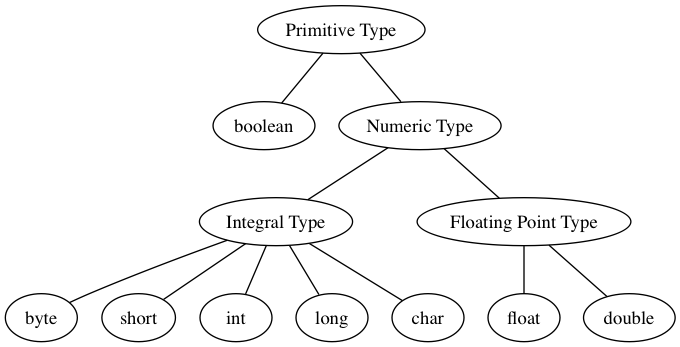
\includegraphics[width=\linewidth]{primitives.png}
\caption{Primitive Classification}
\label{fig:results}
\end{figure}

Java specification\cite{gosling} defines sizes and ranges for primitive types. The integer types are clear cut, but the floating point types are not so simple. They follow the ANSI/IEEE Standard 754-1985\footnote{see http://docs.oracle.com/javase/specs/jls/se7/html/jls-4.html\#jls-4.2.3 for details}. The values in table~\ref{tab:java-primitive-types} are from my MacBookPro, printing out the max value for float and double. They might be different on a different architecture.

Also to note that although Java defines the primitive sizes, on different architectures might actually use different sizes. For example, although an int is defined as 32 bits, it might take 64 bits on a 64 bit computer. The primitive sizes defined in the Java Specification is how the programmer sees the types, not necessarily how they are stored.

The list of primitives in Java\cite{gosling}:
\begin{table}[!htb]
\centering
\begin{tabulary}{\columnwidth}{ |>{\raggedright\arraybackslash} p{0.15\columnwidth} | >{\raggedright\arraybackslash}p{0.1\columnwidth} | >{\raggedright\arraybackslash}p{0.59\columnwidth} |}
\hline
\textbf{Type} & \textbf{Size (bits)} & \textbf{Range} \\ \hline 
byte  & 8  & from -128 to 127, inclusive \\ \hline 
short & 16 & from -32768 to 32767, inclusive \\ \hline 
int   & 32 & from -2147483648 to 2147483647, inclusive \\ \hline 
long  & 64 & from -9223372036854775808 to 9223372036854775807, inclusive \\ \hline
char  & 16 & from '\textbackslash{}u0000' to '\textbackslash{}uffff' inclusive, that is, from 0 to 65535 \\ \hline 
float & 32 & from -3.4028235E38 to 3.4028235E38\footnotemark[3] \\ \hline
double & 64 &from -1.7976931348623157E308 to 1.7976931348623157E308\footnotemark[3] \\ \hline
boolean & 32\footnotemark[4] & true or false \\ \hline
\end{tabulary}
\caption{Java Primitive Types}\label{tab:java-primitive-types}
\end{table}

\footnotetext[3]{Java float and double follow the  ANSI/IEEE Standard 754-1985, see http://docs.oracle.com/javase/specs/jls/se7/html/jls-4.html\#jls-4.2.3}
\footnotetext[4]{\texttt{boolean} is internally implemented like an \texttt{int}}
\subsubsection{Heap and Stack}
Java virtual machine memory is divided into two types; stack and the heap. Each thread gets its own stack. The heap is shared. The stack is divided into frames, which contain slots for data, called local variables, and other things. There is one frame per method call.

The The Java® Virtual Machine Specification doesn't actually specify where the different data types are stored. It specifies that the stack can store data that is needed. The frames in the stack can be heap allocated.

Usually, though, in the past the stack is used for storing primitive data, addresses to the heap, and return data. The heap holds more complex information, such as objects and arrays. A good rule of thumb is that if you create something using the keyword "new" it will end up in the heap.

Primitives are stored in the stack. Types boolean, byte, char, short, int, and float occupy one "local variable" slot in the stack frame. Types long or double occupy two slots. \cite{gosling}
\begin{figure}[H]\centering
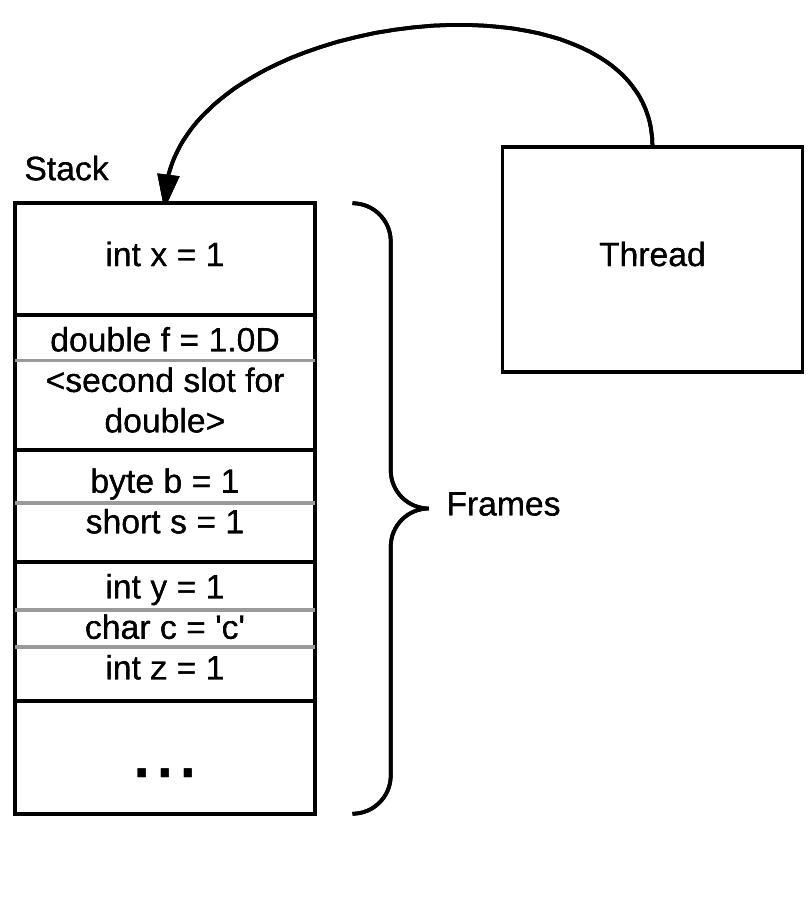
\includegraphics[width=0.9\linewidth]{images/stack}
\caption{The Stack}
\label{fig:stack}
\end{figure}
Figure \ref{fig:stack} depicts a thread with a stack that has four frames in it. The first frame has one primitive stored in it (an integer). The second one has one double, that takes up two "local variable" slots. The third and fourth frame have two and three primitives, respectively.

\subsubsection{Class With Fields on the Heap}
The stack is for simple data, like the primitives. They take up a predefined space of space. Objects are variable in size. Even two objects, created from the same class can be different in size. Objects cannot be stored in the stack, they are stored in the heap.

The reference to the object is stored in the stack. The reference points to an address in the heap, which contains the class and its fields.\cite{gosling}
\begin{figure}[H]\centering
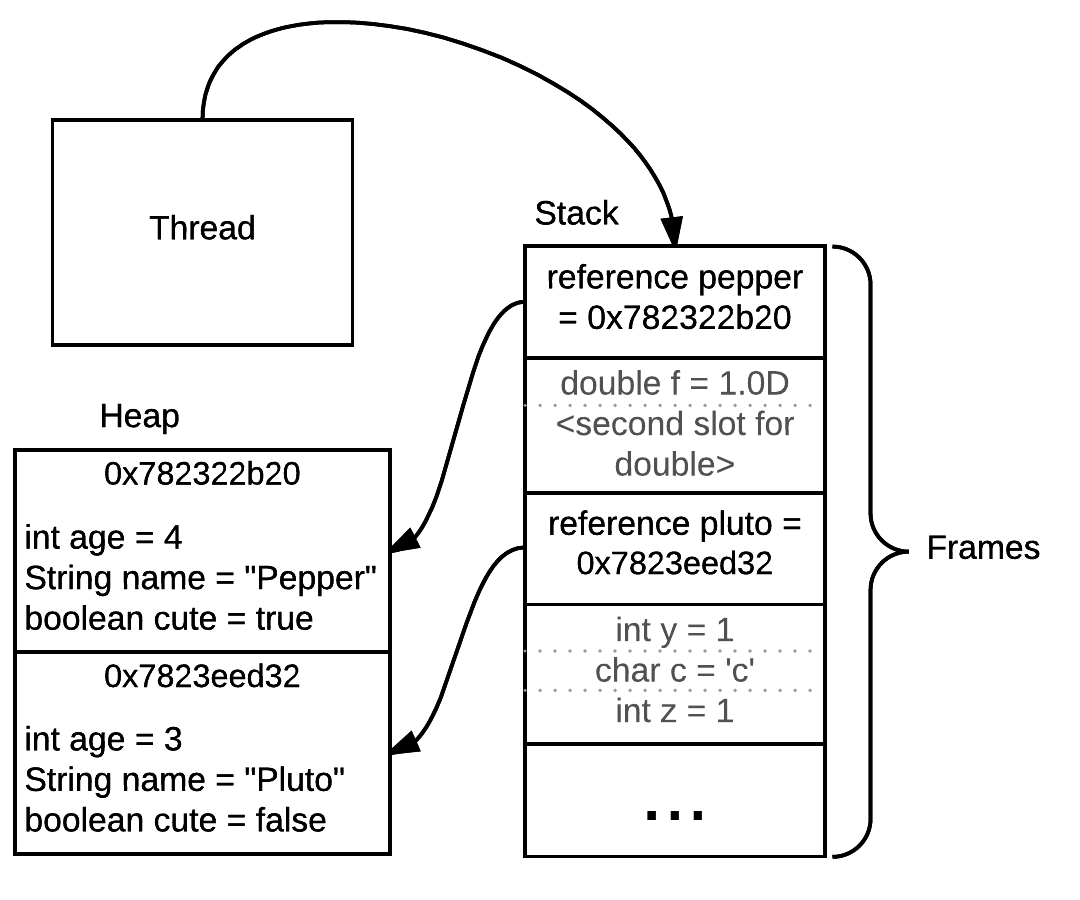
\includegraphics[width=0.9\linewidth]{images/heap}
\caption{The Heap}
\label{fig:stack}
\end{figure}
\subsubsection{String Storage} in Java is represented by sequences of Unicode code points. String is a sequence of characters, which each is represented by two bytes. 

a Java String is a special creature. You can create it as a literal:
\begin{lstlisting}[language=Java]
String literalStr = "test";
\end{lstlisting}
or as an Object:
\begin{lstlisting}[language=Java]
String newStr = new String("test");
\end{lstlisting}

In both cases the reference to it is stored in the stack, the actually string data is in the heap.

Those two strings are additionally curious, though. The literal string is created as an internal string. That means that there is only one copy of the literal string.

Consider the following
\begin{lstlisting}[language=Java]
String newStr      = new String("test");
String newStr2     = new String("test");
String newStr3     = newStr;
String literalStr  = "test";
String internalStr = newStr.intern();
\end{lstlisting}

We can compare these strings in two ways. We can see if the actual characters are the same, or if they actually are the same object (the reference in the stack points to the same spot in the heap).

Comparing newStr and newStr2:
\begin{lstlisting}[language=Java]
newStr      and newStr2     are  not the same
newStr      and newStr2     are  equal
\end{lstlisting}

We created two objects, with exactly the same contents. They are equal (characters match) but not the same (references do not match).

Comparing newStr and newStr3:
\begin{lstlisting}[language=Java]
newStr      and newStr3     are  the same
newStr      and newStr3     are  equal
\end{lstlisting}

We created one object (newStr) and assigned the same reference to the other (newStr3). The values are equal and also the same. There are two values in the stack that point to the same spot in the heap. Changing the contents of one will also affect the other because they are the same.

Comparing newStr and literalStr:
\begin{lstlisting}[language=Java]
newStr      and literalStr  are  not the same
newStr      and literalStr  are  equal
\end{lstlisting}

They are equal (characters match) but they are not the same, as expected. There are two different strings in the heap.

How about the newStr and the internalStr:
\begin{lstlisting}[language=Java]
newStr      and internalStr are  not the same
newStr      and internalStr are  equal
\end{lstlisting}

Just like the previous comparison with the literalStr, internalStr is equal to newStr, but they are not the same.

Now the interesting test, literalStr and internalStr. Notice how internalStr is created from newStr by requesting its internal representation. The results of the comparison:
\begin{lstlisting}[language=Java]
literalStr  and internalStr are  the same
literalStr  and internalStr are  equal
\end{lstlisting}

They are equal and they point to the same location in the heap.

Strings in Java are immutable. Their values cannot be changed. We can assign a new value to a String reference, though. In effect, the string changes, but it really points to a new location in the heap.

The exact location of the internal (literal) strings in the heap used to be different. In Java7 it data changed\cite{java7}:

\begin{quotation}
In JDK 7, interned strings are no longer allocated in the permanent generation of the Java heap, but are instead allocated in the main part of the Java heap (known as the young and old generations), along with the other objects created by the application. This change will result in more data residing in the main Java heap, and less data in the permanent generation, and thus may require heap sizes to be adjusted. Most applications will see only relatively small differences in heap usage due to this change, but larger applications that load many classes or make heavy use of the String.intern() method will see more significant differences.
\end{quotation}


\subsubsection{Storing an Array of ints or Objects}
An Array is an Object that contains other things that are homogeneous. All items in an Array must be of the same type. An Array could, for example, contain ints or Objects (of the same type). 

Regardless of what is stored in the Array, because it is an Object, it is stored like an Object. A reference to it is in the stack, and the actual contents are in the heap.